In this chapter we will investegate the effect of the Boussinesq approximation on the simulations.

\section{Steady state profiles}
%
\begin{figure}[h]
    \centering
    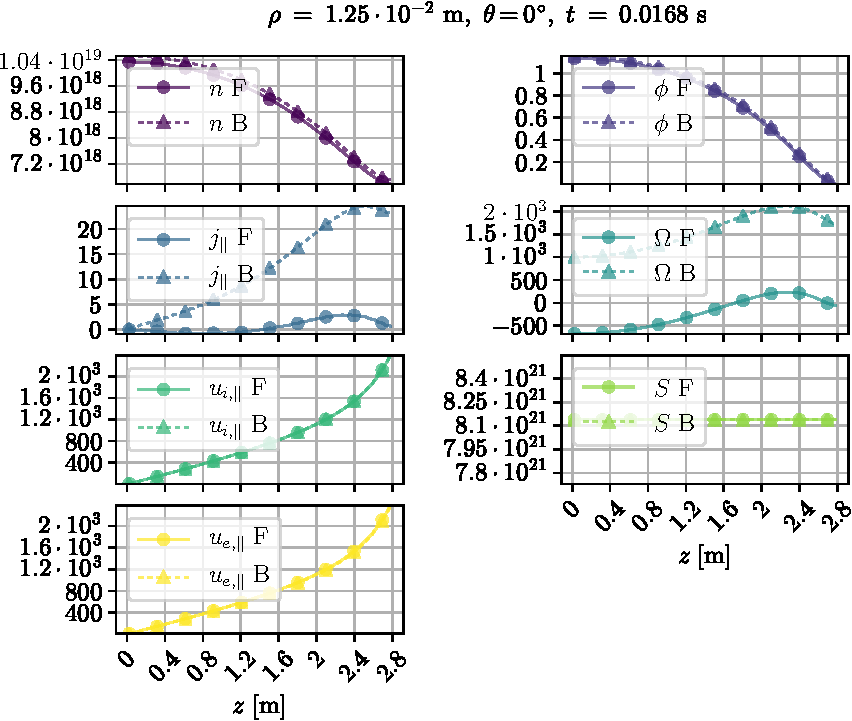
\includegraphics[width=1.0\textwidth]{fig/results/compareBouss/1DProfRad001B}
    \caption{Radial steady state profiles with and without the Boussinesq approximation.}
    \label{fig:compareBoussProfRad}
\end{figure}
%
We note that any difference between the model using the Boussinesq approximation, and the one which do not, lays in the vorticity equation.
The biggest difference between \cref{eq:celma_vortD_evolution} and \cref{eq:celma_vort_boussinesq} is how the density factor in the compression of the density times the ion polarization term is treated.
When we used the Boussinesq approximation, we assumed that this $n$ was the same as a flat background $n_0$, which disappeared from the equations when we normalized.
This left us with a source term.
The source terms does not appear in the non-Boussinesq case as it cancels with the source term from the density equation which we "smuggled" inside the $\d_t^E$ operator.
Finally, the $\ve{E}\times\ve{B}$ advection terms are different in the two cases.
These differences affects both the background profiles and terms affecting the fluctuations.

Thus, there should come as no surprise that the radial vorticity profile has changed, as indicated in \cref{fig:compareBoussProfRad}.
This in turn changes the radial potential profile%
%
\footnote{One could say that it is the potential which determines the vorticity through $\Om = \grad_\perp^2 \phi$, but since we are evolving the vorticity in time we are instead inverting the equation for $\phi$.
In that respect $\Om$ determines $\phi$.}%
%
.
The radial density profile and the radial parallel velocity profiles stays roughly the same, albeit with slower parallel velocities close to $L_\rho = \rho$.
This, in turn, makes small changes in the radial parallel current profile, but gives a more shallow approach to $\rho=L_\rho$.
%
\begin{figure}[h]
    \centering
    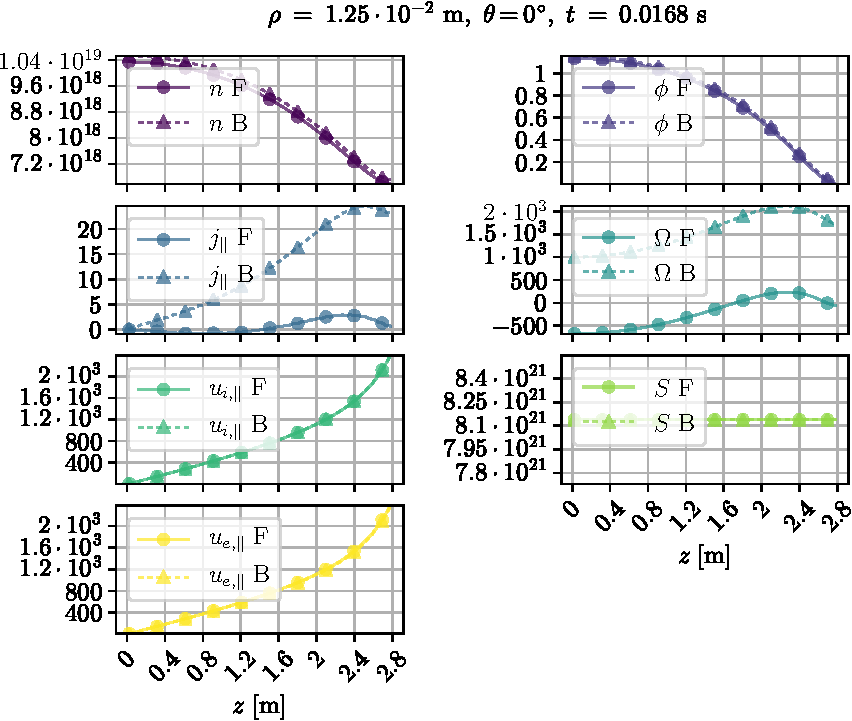
\includegraphics[width=1.0\textwidth]{fig/results/compareBouss/1DProfPar001B}
    \caption{Parallel steady state profiles with and without the Boussinesq approximation.}
    \label{fig:compareBoussProfPar}
\end{figure}
%
On the other side, the parallel parallel current profile has changed, as seen in \cref{fig:compareBoussProfPar}.
First of all, the see-sawing seen in the non-Boussinesq case seem to have disappeared.
Although the oscillating patterns in the parallel current is still there, they are much less pronounced due to the higher values of $j_\|$.
Secondly the parallel current is around $5$ time larger in magnitude close to the sheath entrance.
This comes from that the balancing terms in the vorticity equation has changed.
In the non-Boussinesq case, the $n$ in $\div(nu_{p,i})$ helped to reduce the terms in the modified vorticity, and thereby the parallel current as $n$ was lower closer to the sheath.
As mentioned above, this $n$ disappears when using the Boussinesq approximation, so it can no longer help to reduce the parallel current.
We can see that this change cannot have its origin in the $\ve{E}\times\ve{B}$ advection terms, as these are not active during the steady state since the $\phi$-field is axisymmetric.
Neither can it origin from the additional source term due to the lack of $n$ dependence.
We can also observe that although the shape of the parallel vorticity profile is more or less equal, is does not cross zero as is the case in the non-Boussinesq case.
Finally, it is worth noting that the system still follows a Boltzmann distribution to a high degree, as is the case in the non-Boussinesq case.
%

\section{The linear state}
%
The change in the vorticity equation has a profound effect on the growth rates in the linear phase.
This is illustrated in \cref{fig:compFFTB}.
%
\begin{figure}[h!]
    \centering
    \begin{subfigure}[h]{0.45\textwidth}
        \centering
        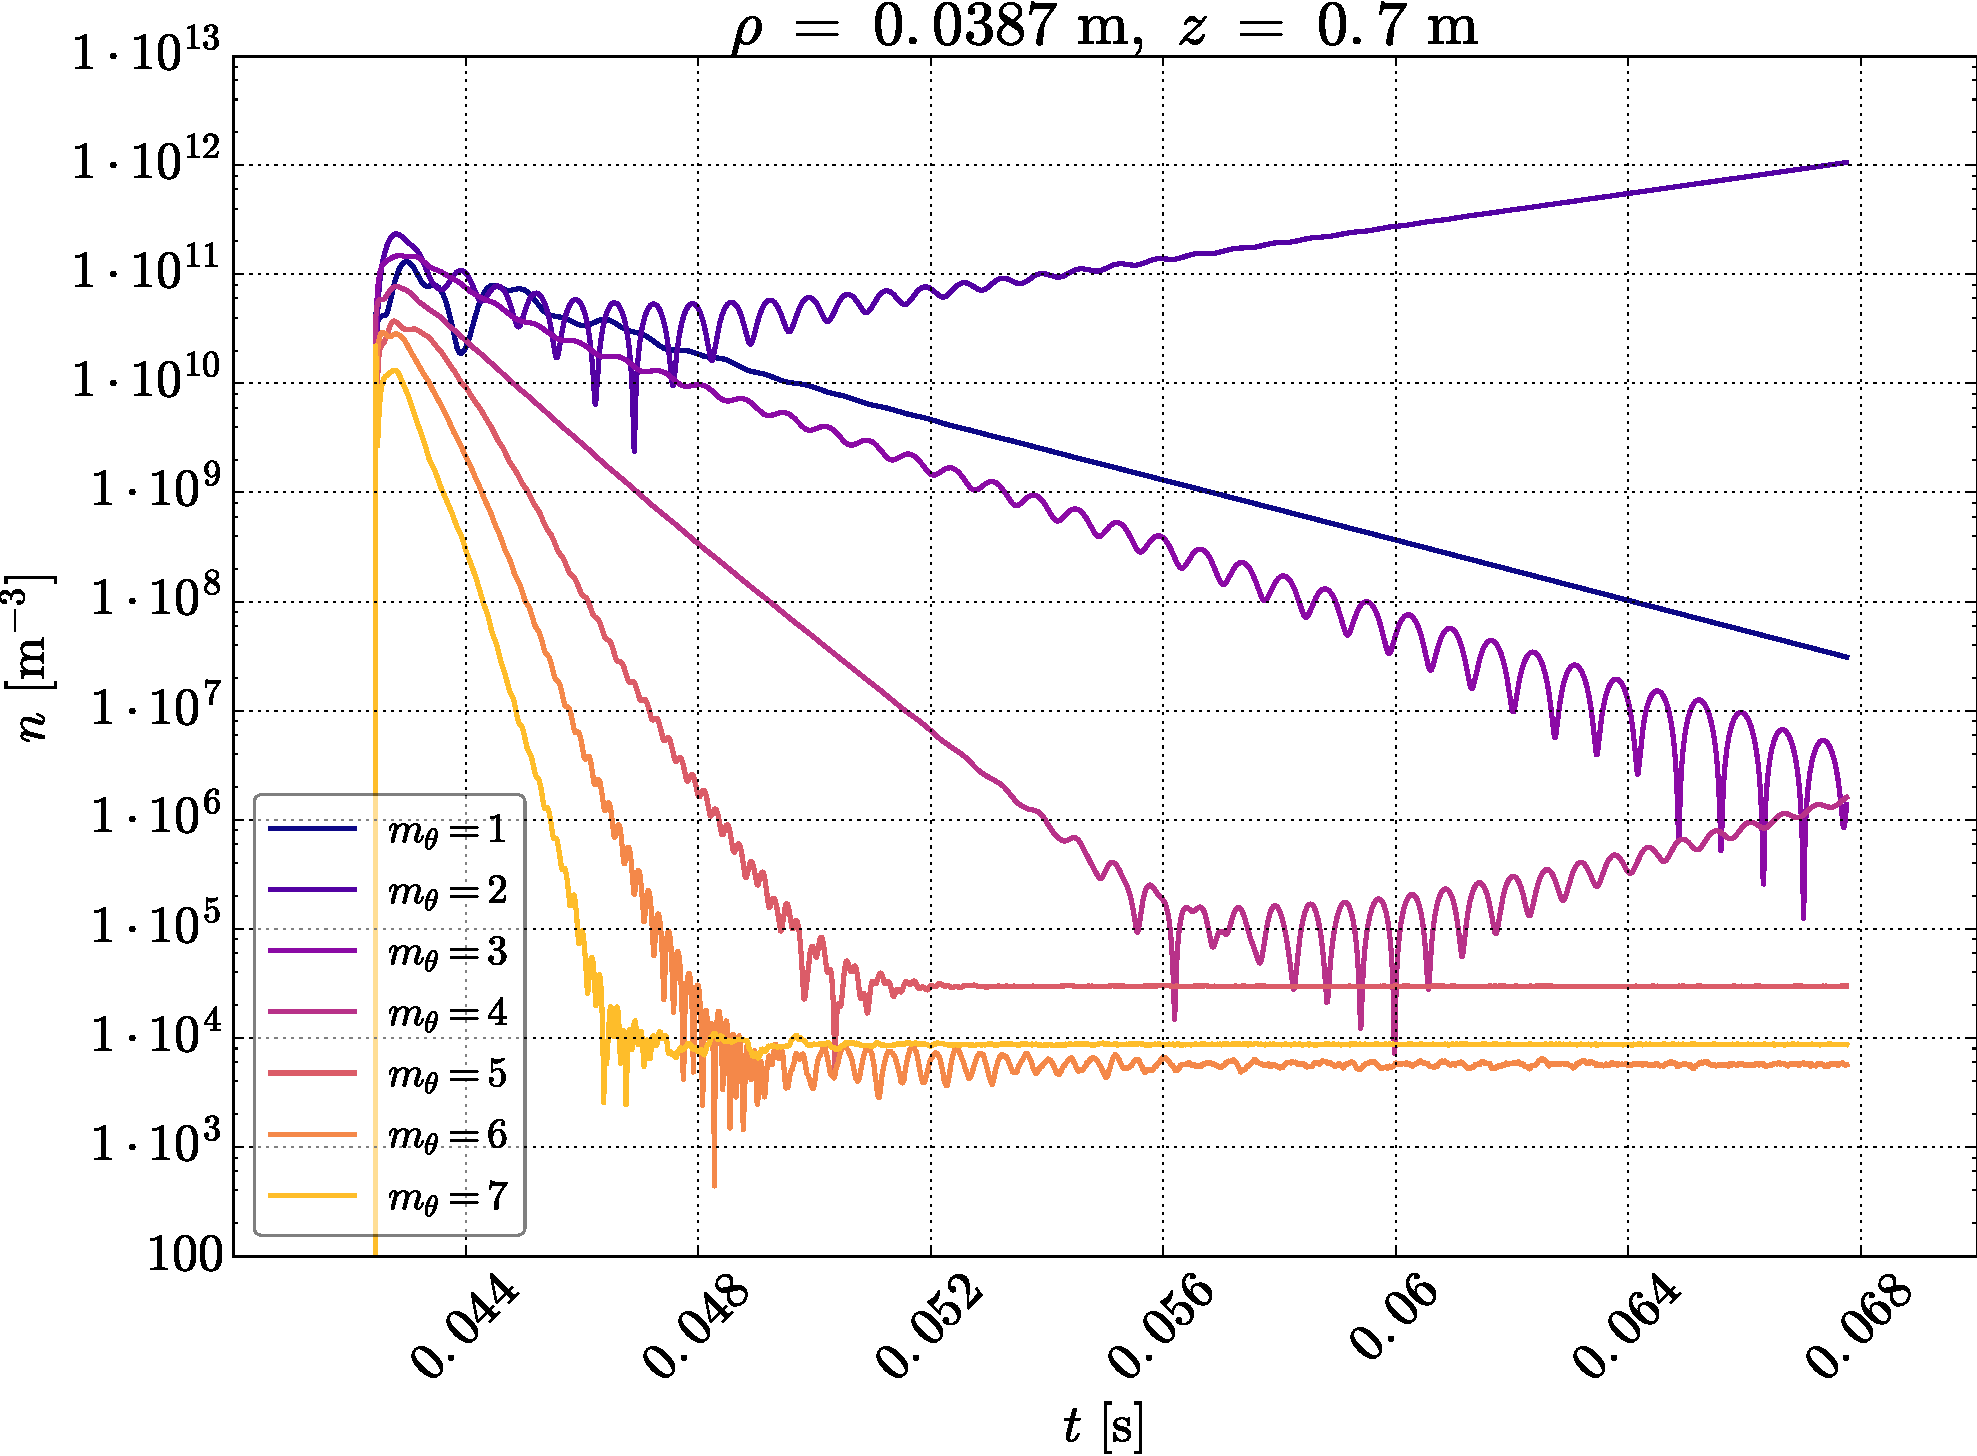
\includegraphics[width=1.0\textwidth]{fig/results/compareBouss/FFT004}
        \caption{Without the Boussinesq approximation}
        \label{fig:FFTWOB}
    \end{subfigure}%
    \hfill
    \begin{subfigure}[h]{0.45\textwidth}
        \centering
        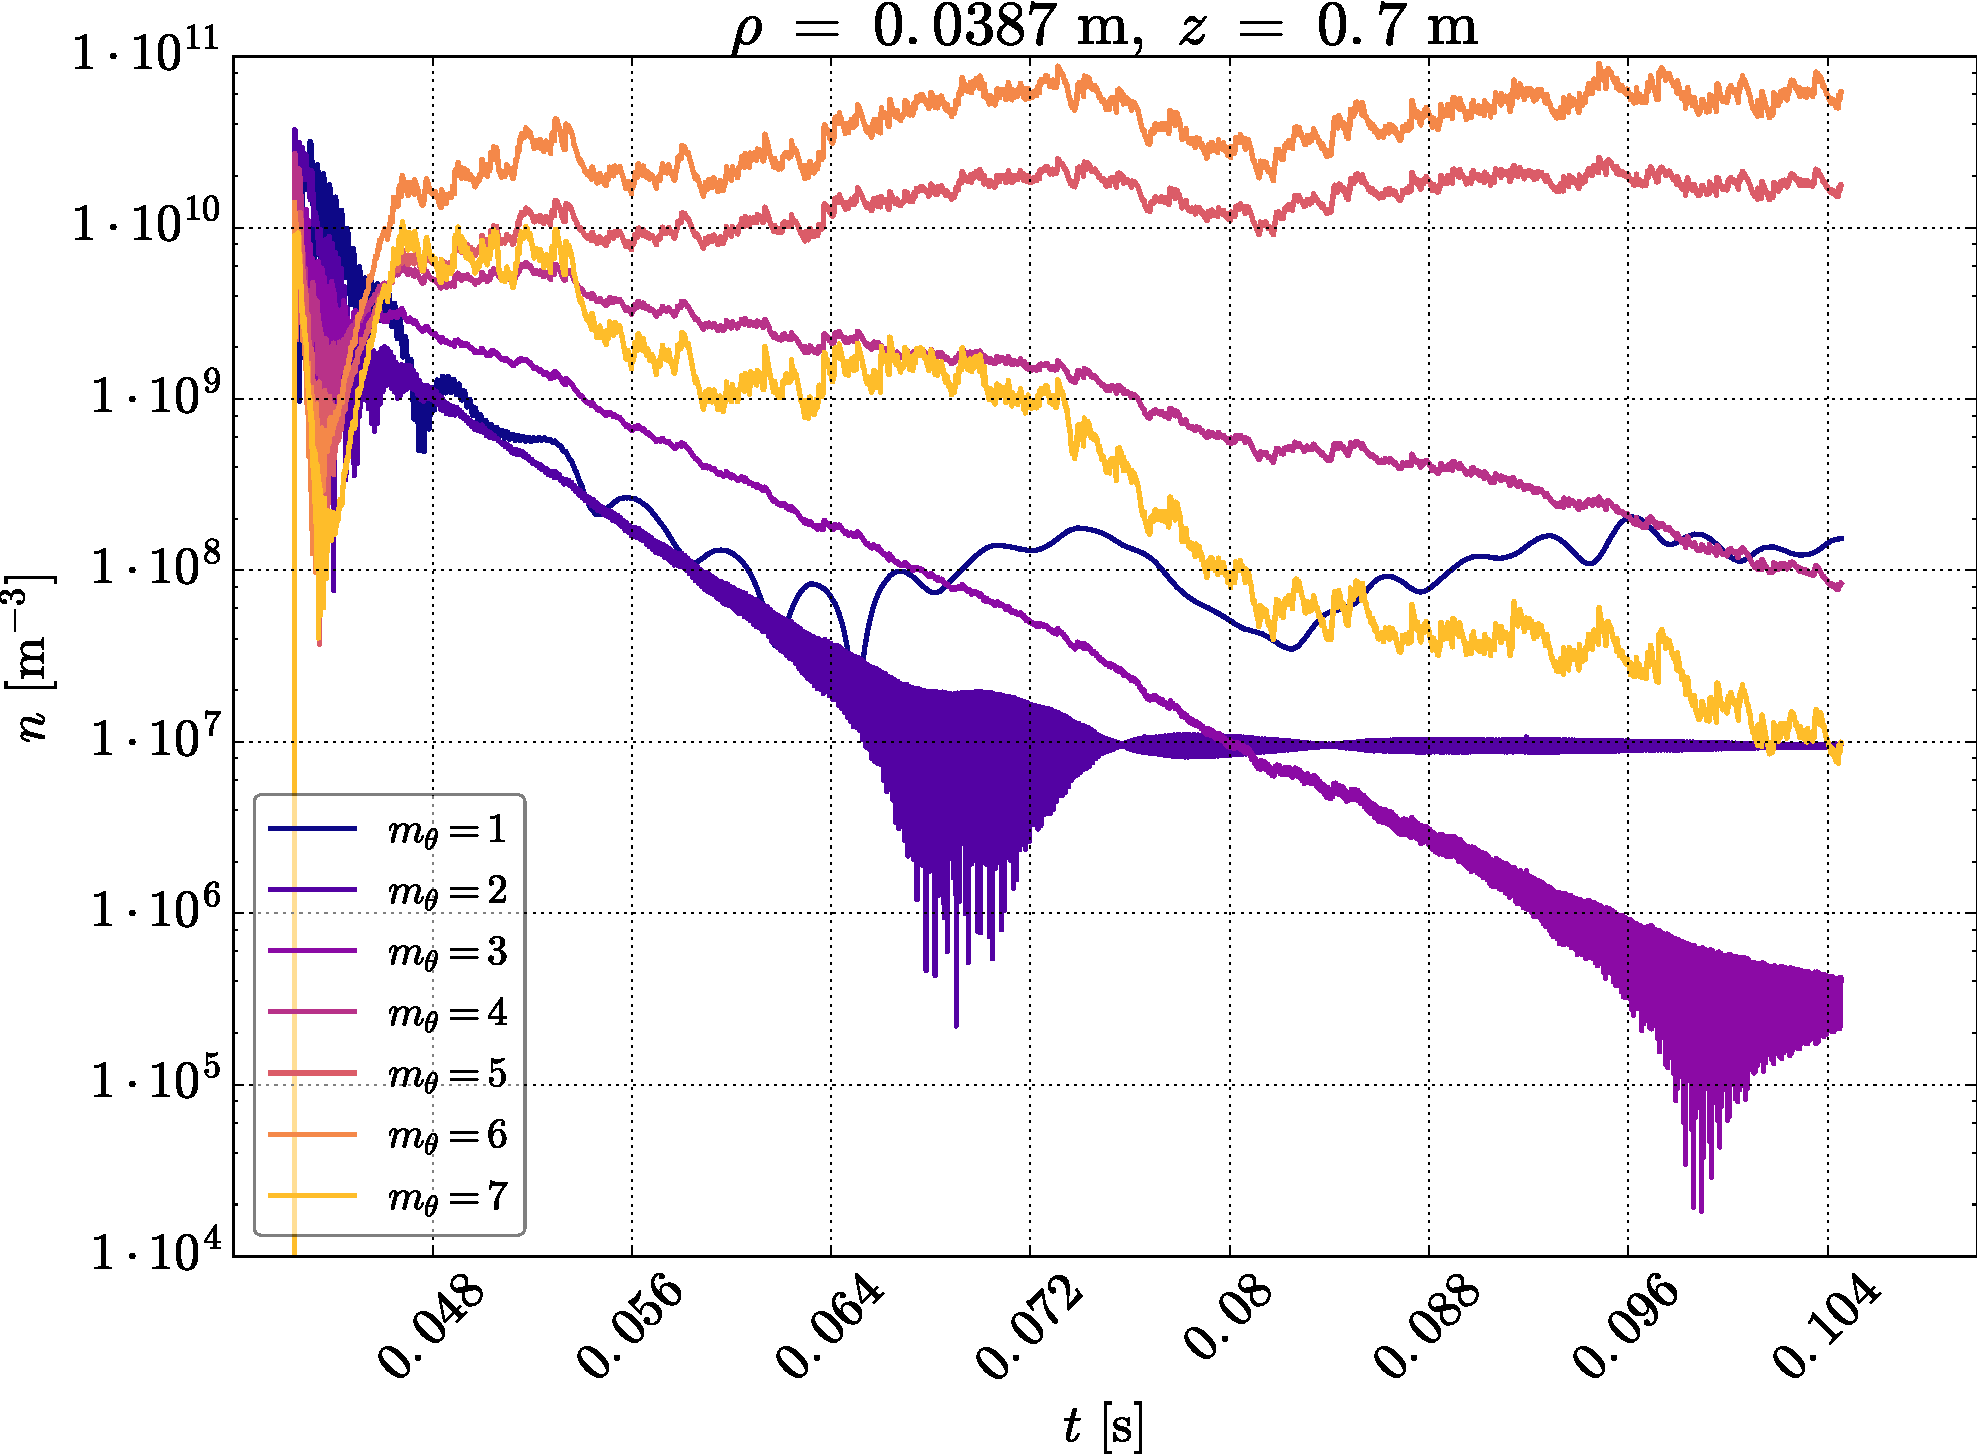
\includegraphics[width=1.0\textwidth]{fig/results/compareBouss/FFT004B}
        \caption{With the Boussinesq approximation.}
        \label{fig:FFTWB}
    \end{subfigure}
    \caption{Fourier modes of the density at $B=0.04\T$}
    \label{fig:compFFTB}
\end{figure}
%
While the \nth{2} mode grows in the non-Boussinesq case, no mode seems to be exponential growing when using the Boussinesq approximation.
%
\begin{figure}[h]
    \centering
    \begin{subfigure}[h]{0.5\textwidth}
        \centering
        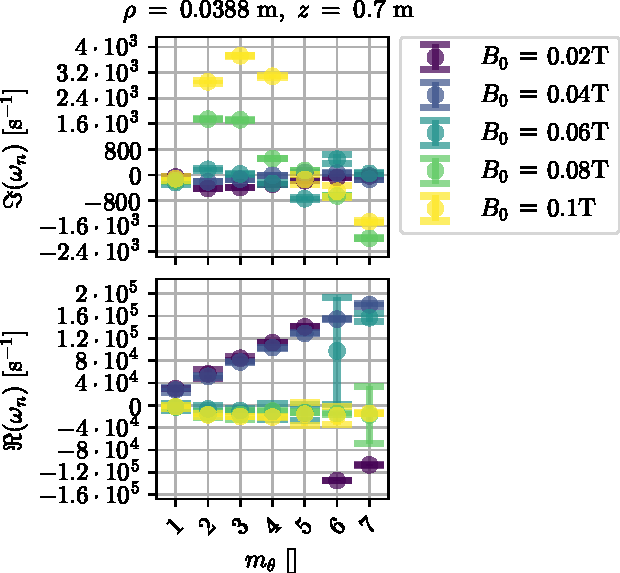
\includegraphics[width=1.0\textwidth]{fig/results/compareBouss/growthRatesB0Bous}
        \label{fig:grBBous}
    \end{subfigure}%
    \\
    \begin{subfigure}[h]{0.50\textwidth}
        \centering
        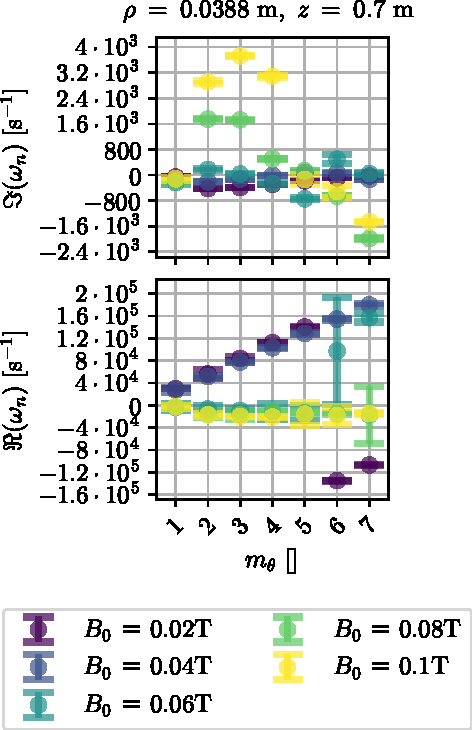
\includegraphics[width=1.0\textwidth]{fig/results/compareBouss/growthRatesB0ModeNr}
        \label{fig:grBModeNrBous}
    \end{subfigure}
    \caption{$B$-dependency on growth rates when using the Boussinesq approximation.}
\end{figure}
%
The difference in the linear growth rates can be further examined by comparing \cref{fig:grBBous, fig:grBModeNrBous} to
we see that the most unstable mode occurs for a lower mode number when using the Boussinesq approximation.
In absolute value the growth rates are around half as steep, and the rotation of the modes are larger with almost an order of magnitude when using the Boussinesq approximation.
% FIXME: Explain why

\section{The turbulence phase}
%
There is also a large differences between the Boussinesq and the non-Boussinesq case in the turbulent state.
When investigating the energy in \cref{fig:energies008B} we notice three things.
%
\begin{figure}[htb]
    \centering
    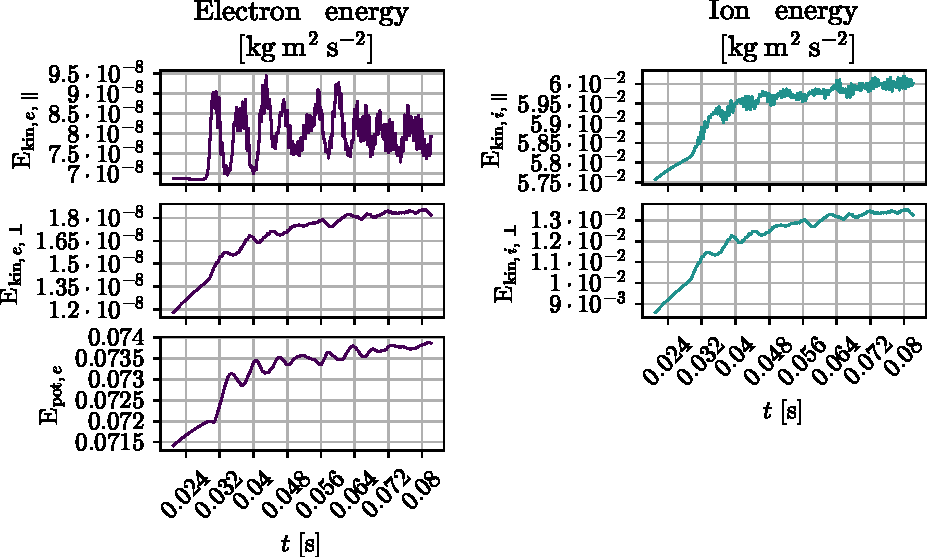
\includegraphics[width=1.0\textwidth]{fig/results/compareBouss/energies008B}
    \caption{Time trace of the energy for $B=0.08\T$ using the Boussinesq approximation.}
    \label{fig:energies008B}
\end{figure}
%
Firstly, in contrast to what is observed in simulations without the Boussinesq approximation, the energy is increasing in the linear phase (with exception of the parallel electron energy, which after close inspection actually shows a slight decrease in the linear phase).
For the potential energy, this means that the total number of particles in the system is increasing as the electron temperature is constant.
If the density is increasing, this would also explain why the other energies are increasing as well.
The parallel electron energy can then only be decreasing if the parallel electron velocity is decreasing.

Next, we do not observe the energy overshoot as we did when investigating the simulations without the Boussinesq approximation.
This can also be seen by visual inspection the temporal evolution of the fields.
The dynamics does not appear to be faster during the onset of the turbulence then during the turbulent state.

Finally, the energy appears to be drifting to higher values with time.
In absolute terms, the energy is also larger when using the Boussinesq approximation.

This can also be seen if when investigating the temporal evolution of the fields.

Visual inspection of the fields also shows that the eddies evolve slower in the turbulence phase as when compared to the non-Boussinesq case, and it appear to be rotating clockwise.
This is shown in

INSERT T MAYBE 5 TRACES.

\section{Fluctuations}
%
The rotation of the plasma structure is also apparent in the time traces of $n$ in the three positions around the maximum gradient.
This is shown in \cref{fig:comb008B}.
%
\begin{figure}[htb]
    \centering
    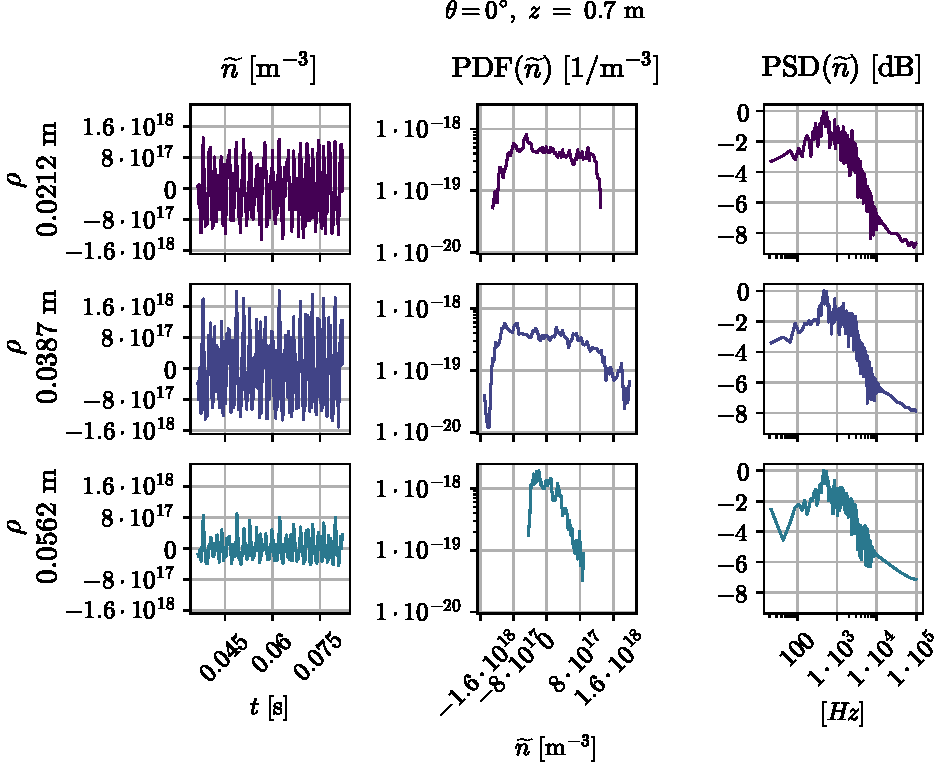
\includegraphics[width=1.0\textwidth]{fig/results/compareBouss/comb008B}
    \caption{Time traces in three fixed positions around the maximum gradient.}
    \label{fig:comb008B}
\end{figure}
%
The fluctuation spectrum is narrower and peaks at a frequency approximately $3$ time as high as compared with the non-Boussinesq case.
We see that flucts are higher in than out, opposite of non-Bouss, due to spinning

The system using the Boussinesq approximation experience less flattening of the profiles as indicated in \cref{}.
Outside the position of the absolute maximum gradient the density profile follows the steady state profile to a good degree.
Furthermore, the potential is shifted closer to the absolute maximum of the gradient.
%
\begin{figure}[htb]
    \centering
    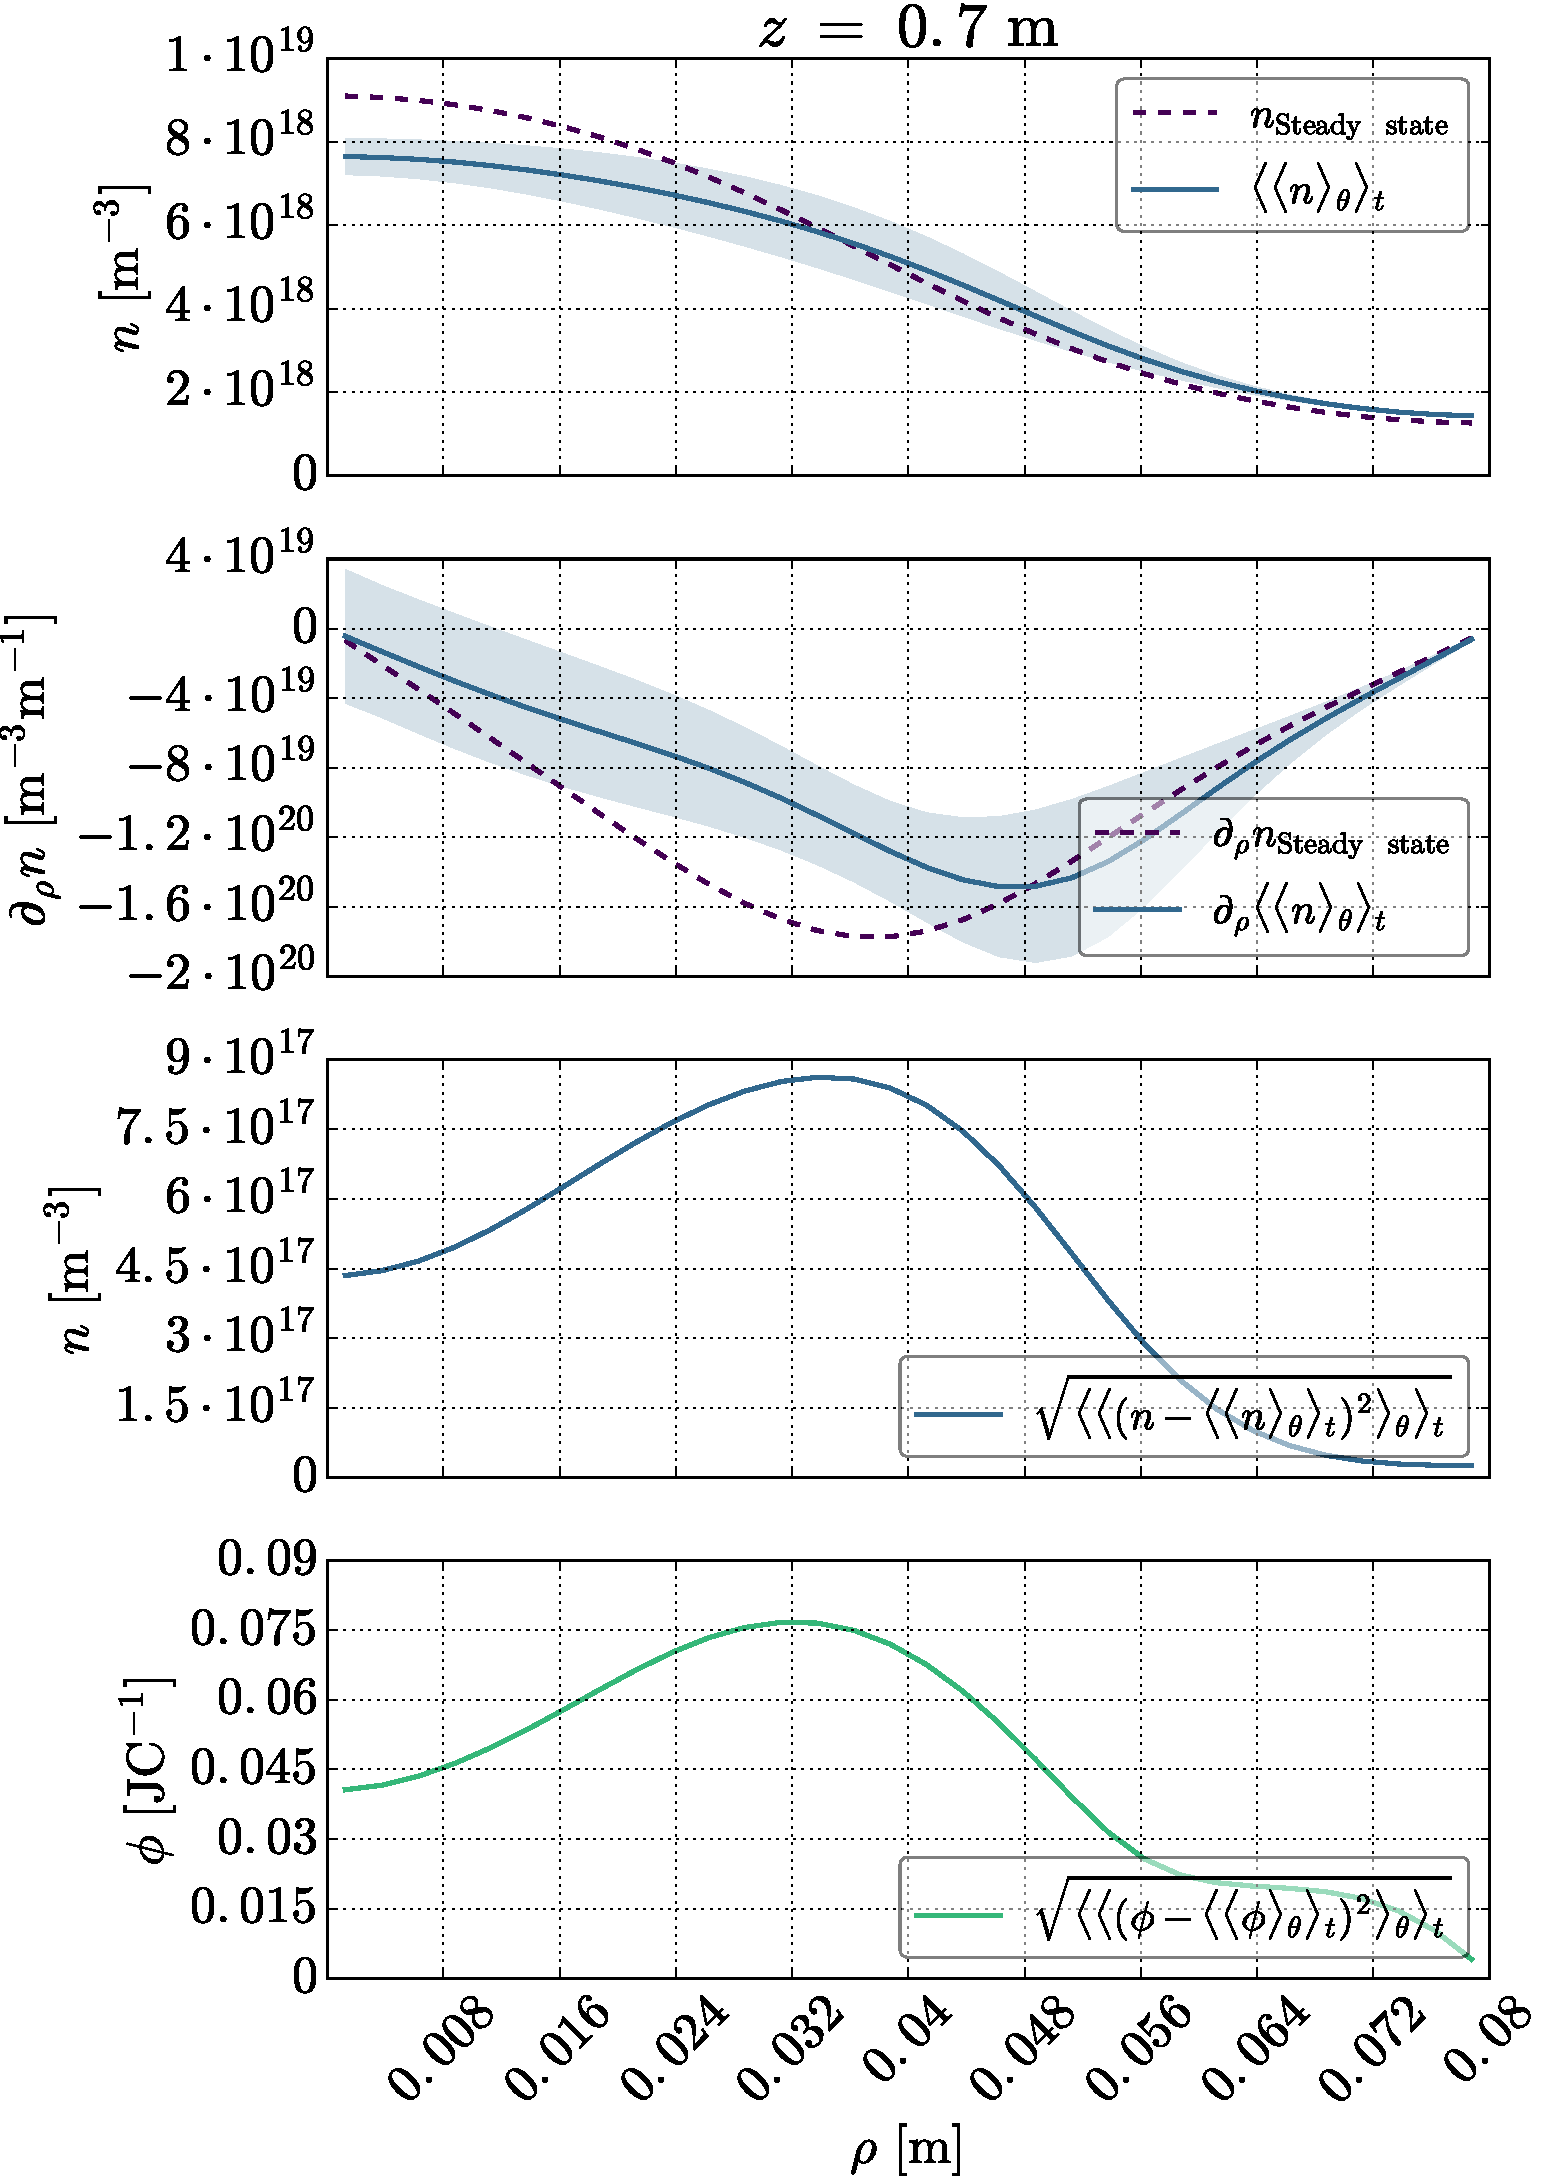
\includegraphics[width=0.45\textwidth]{fig/results/compareBouss/fluctProfiles008B}
    \caption{Steady state and averaged turbulent density profiles together with the radial distribution of the standard deviations of the fluctuations using the Boussinesq approximation with $B=0.08\T$.}
    \label{fig:posOfFluct008B}
\end{figure}
%
Finally, the skewness and kurtosis, shown in \cref{fig:skewKurt008B}, are investigated.
We observe that the system is platikurtic for all radii.
This reflects that the structure rotating around the center of the cylinder has a coherent character.
The skewness is no longer monotonically growing, but has a maximum close to the position of absolute largest gradient of the fluctuating profile.
%
\begin{figure}[htb]
    \centering
    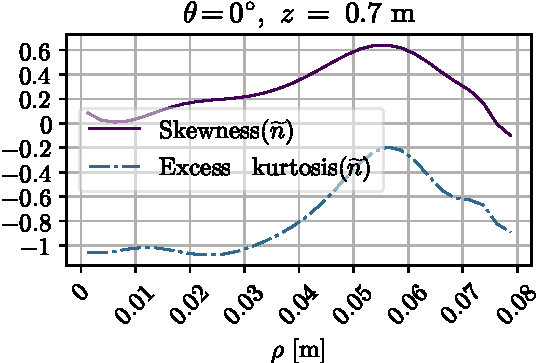
\includegraphics[width=0.45\textwidth]{fig/results/compareBouss/skewKurt008B}
    \caption{Skewness and kurtosis for $B=0.08\T$ using the Boussinesq approximation.}
    \label{fig:skewKurt008B}
\end{figure}
%

\section{Performance comparison}
%
Even though the model without the Boussinesq approximation is more consistent, it comes at a price of increased computation time.
This is shown in \cref{fig:perfB}
%
\begin{figure}[htbp]
    \centering
    \begin{subfigure}[h]{0.45\textwidth}
        \centering
        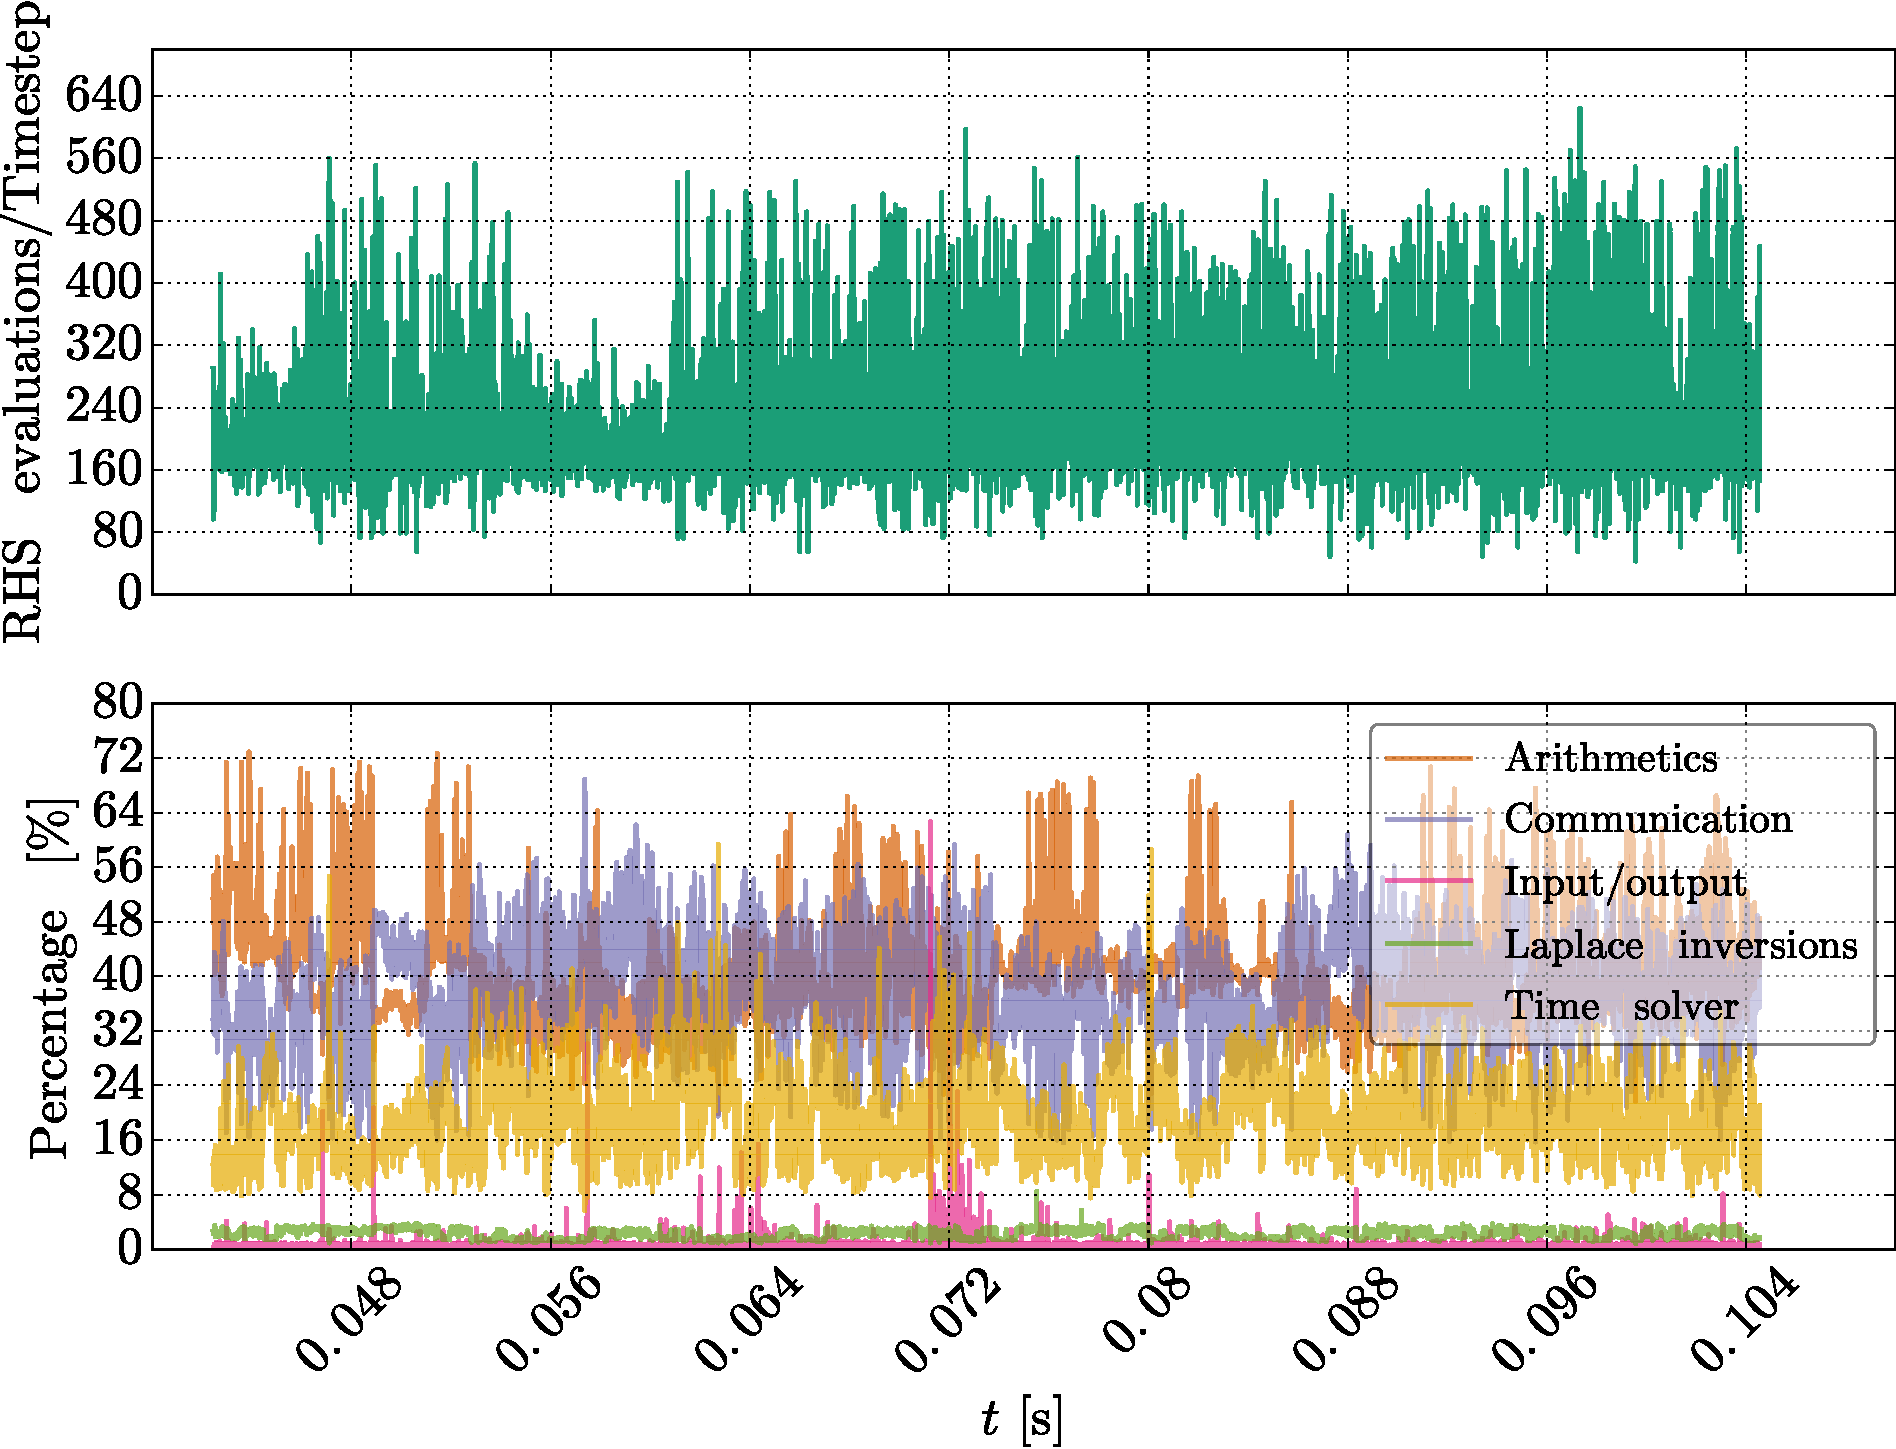
\includegraphics[width=1.0\textwidth]{fig/results/compareBouss/performance004B}
        \caption{$B=0.04\T$}
        \label{fig:perf004B}
    \end{subfigure}%
    \hfill
    \begin{subfigure}[h]{0.45\textwidth}
        \centering
        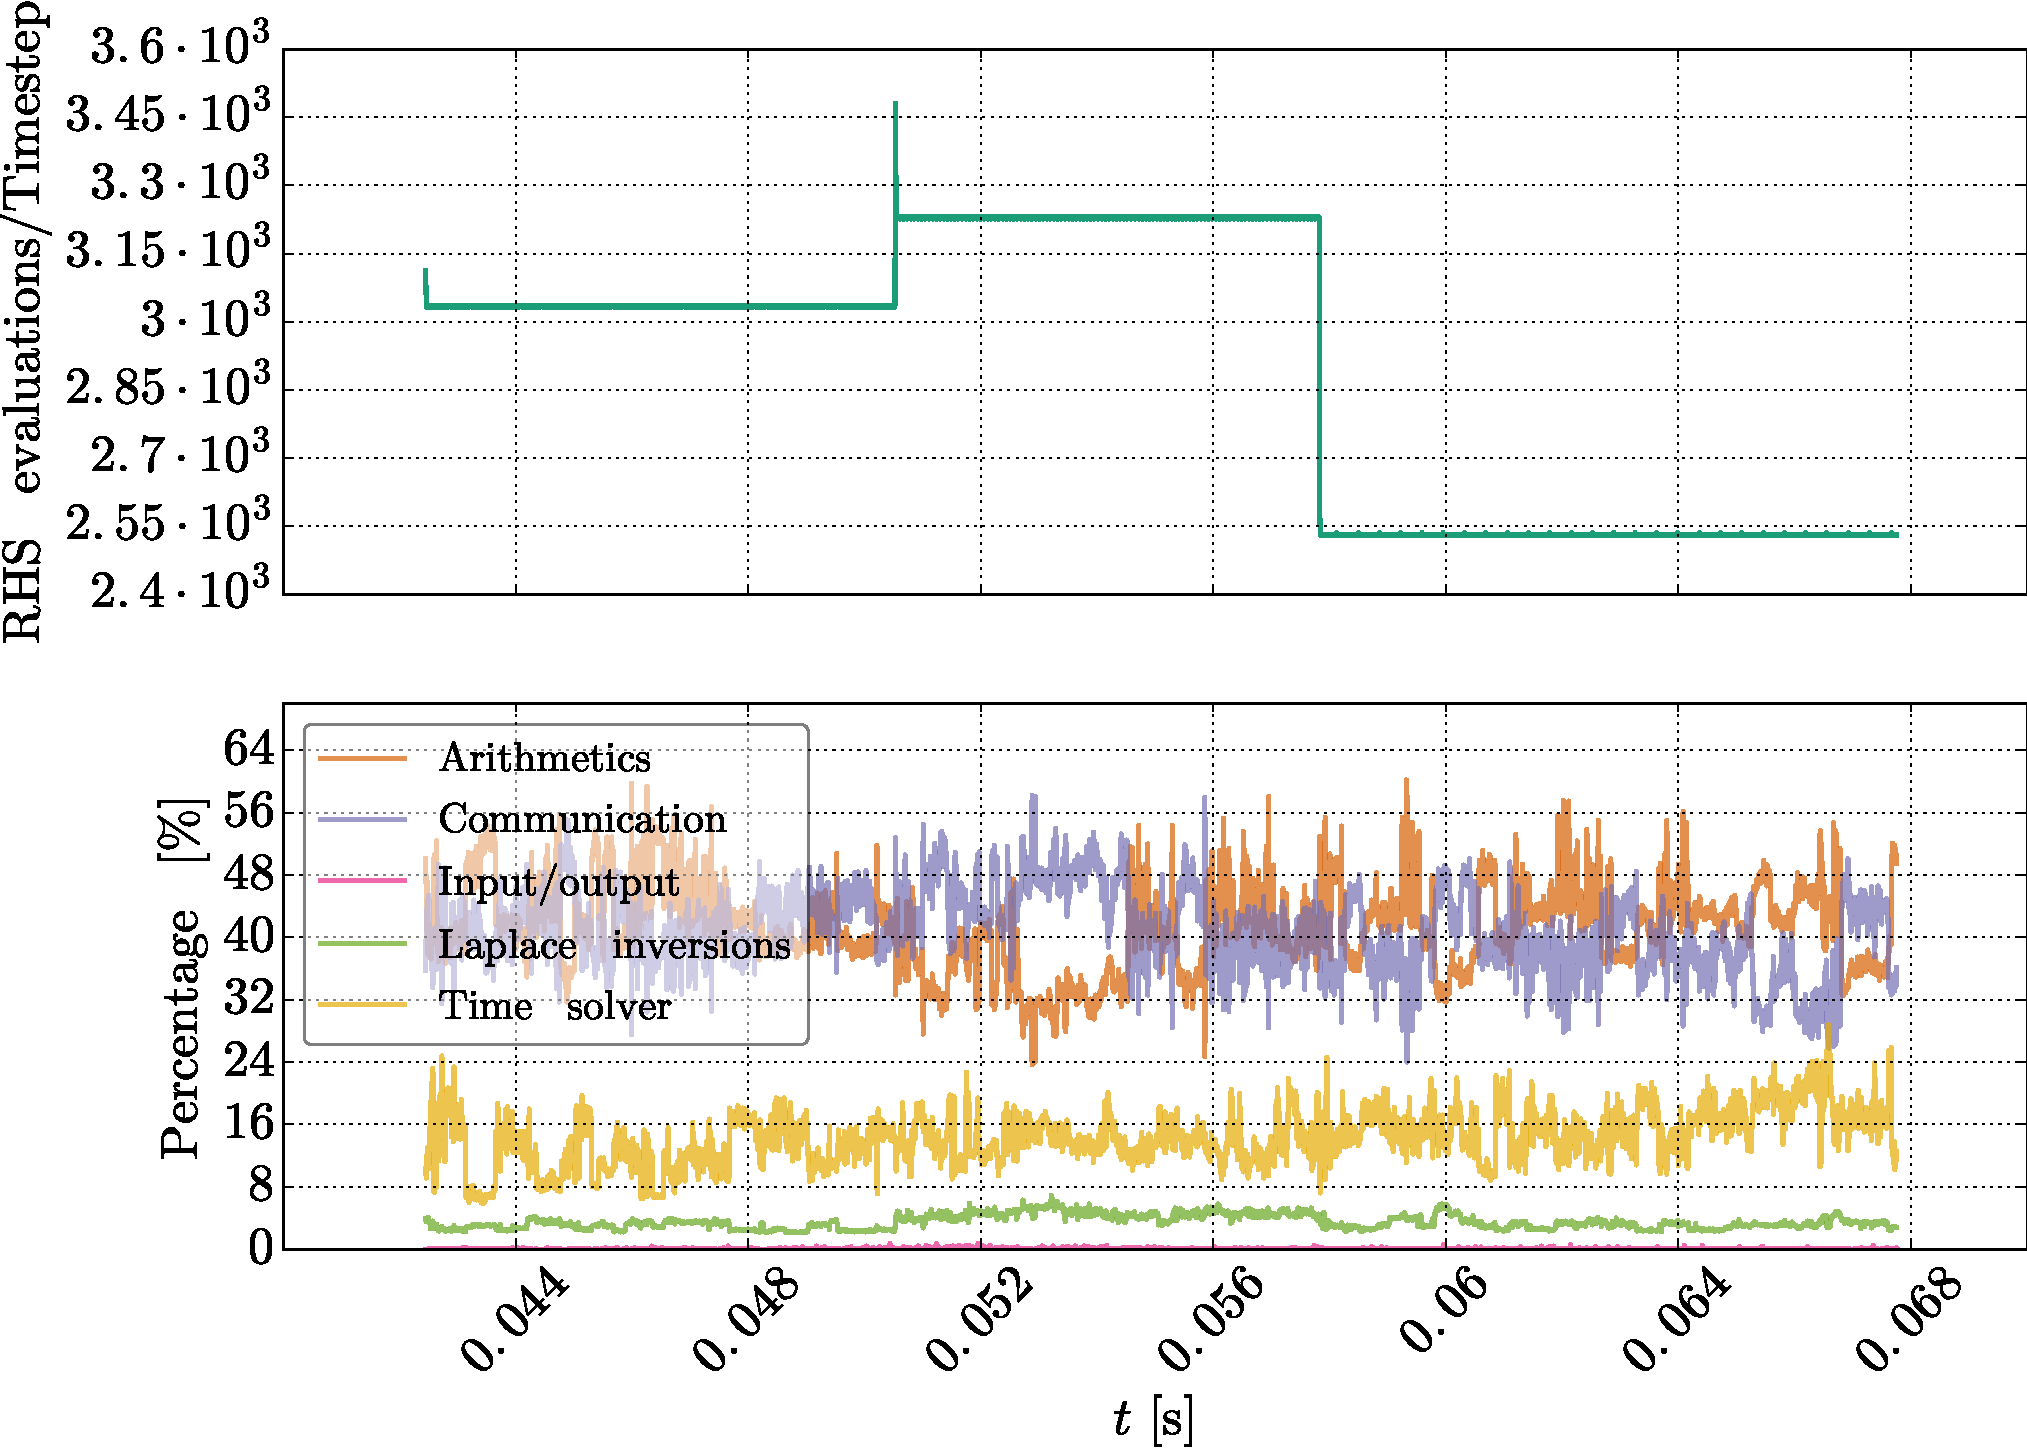
\includegraphics[width=1.0\textwidth]{fig/results/performance/performance004}
        \caption{$B=0.04\T$}
        \label{fig:perf004}
    \end{subfigure}%
    \\
    \begin{subfigure}[h]{0.45\textwidth}
        \centering
        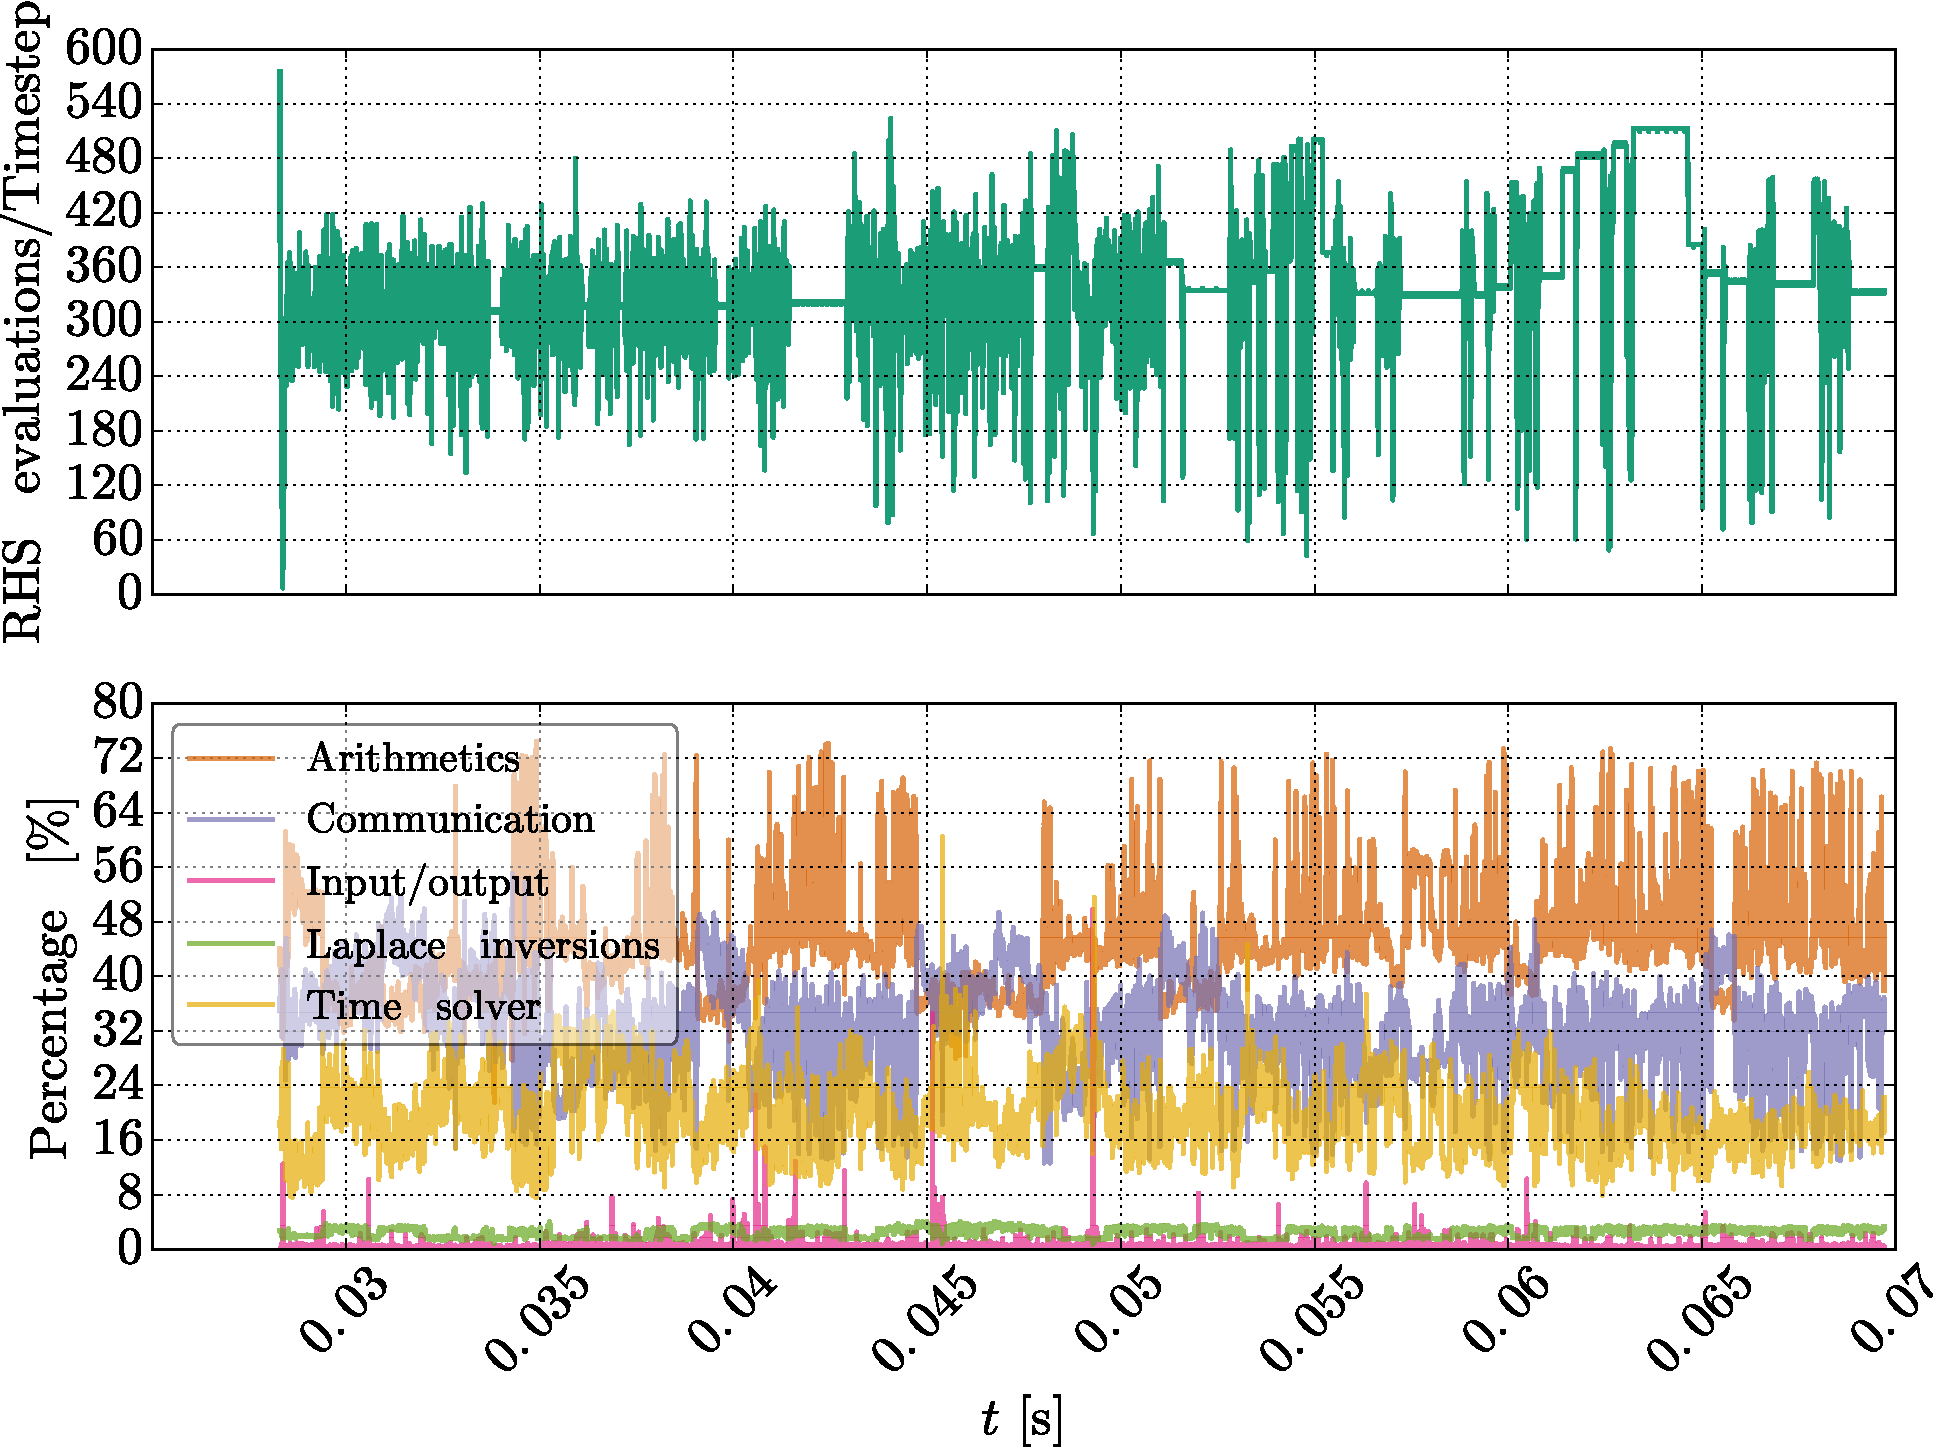
\includegraphics[width=1.0\textwidth]{fig/results/compareBouss/performance006B}
        \caption{$B=0.06\T$}
        \label{fig:perf006B}
    \end{subfigure}
    \hfill
    \begin{subfigure}[h]{0.45\textwidth}
        \centering
        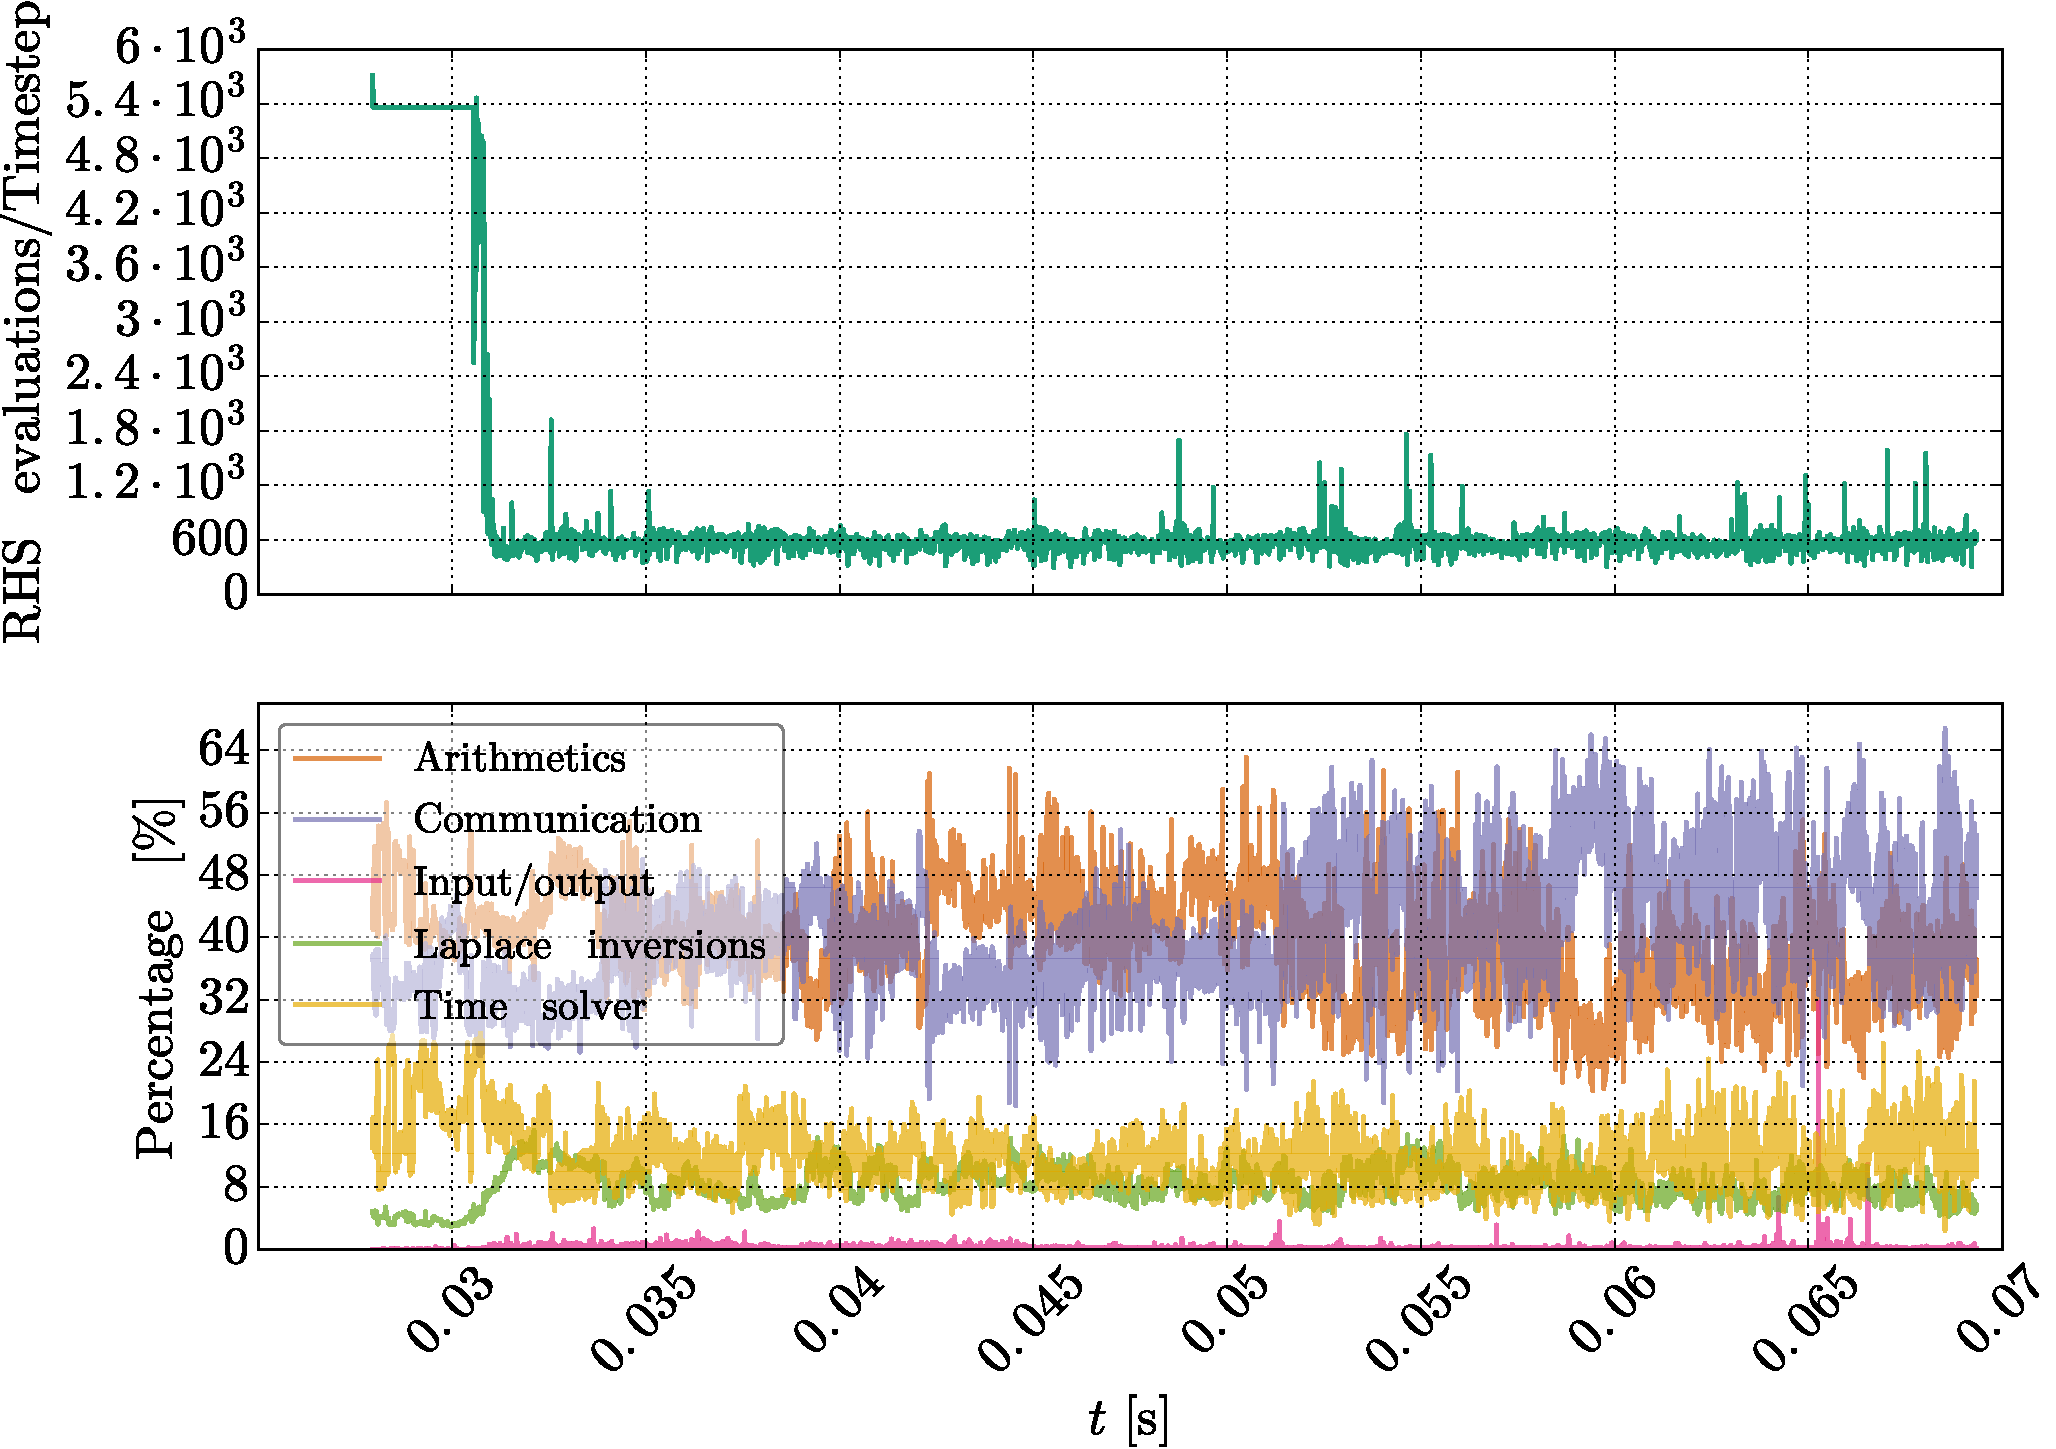
\includegraphics[width=1.0\textwidth]{fig/results/performance/performance006}
        \caption{$B=0.06\T$}
        \label{fig:perf006}
    \end{subfigure}
    \\
    \begin{subfigure}[h]{0.45\textwidth}
        \centering
        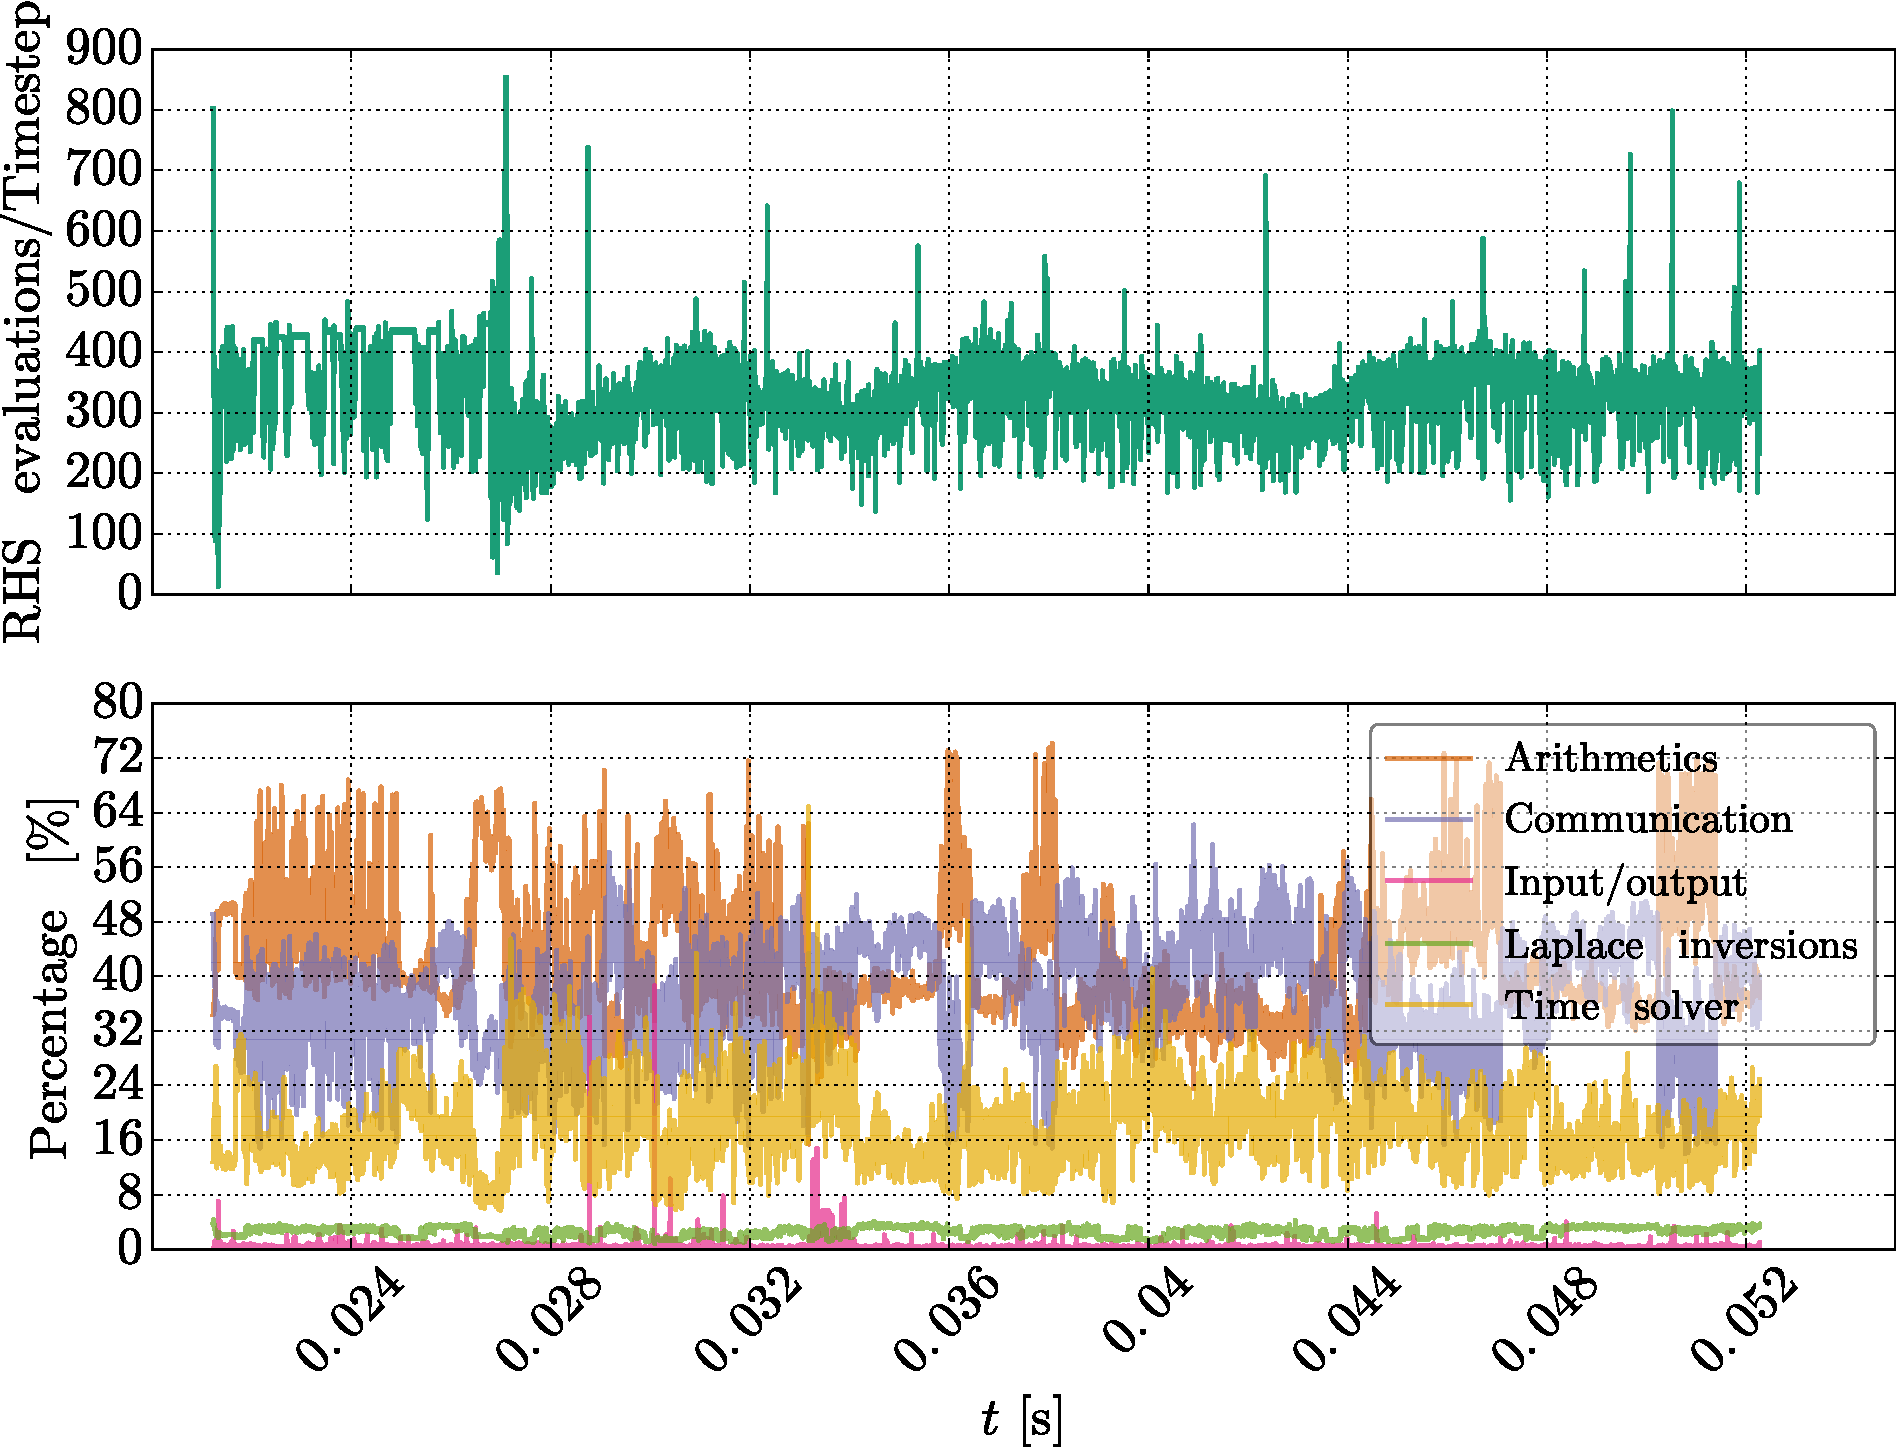
\includegraphics[width=1.0\textwidth]{fig/results/compareBouss/performance008B}
        \caption{$B=0.08\T$}
        \label{fig:perf008B}
    \end{subfigure}
    \hfill
    \begin{subfigure}[h]{0.45\textwidth}
        \centering
        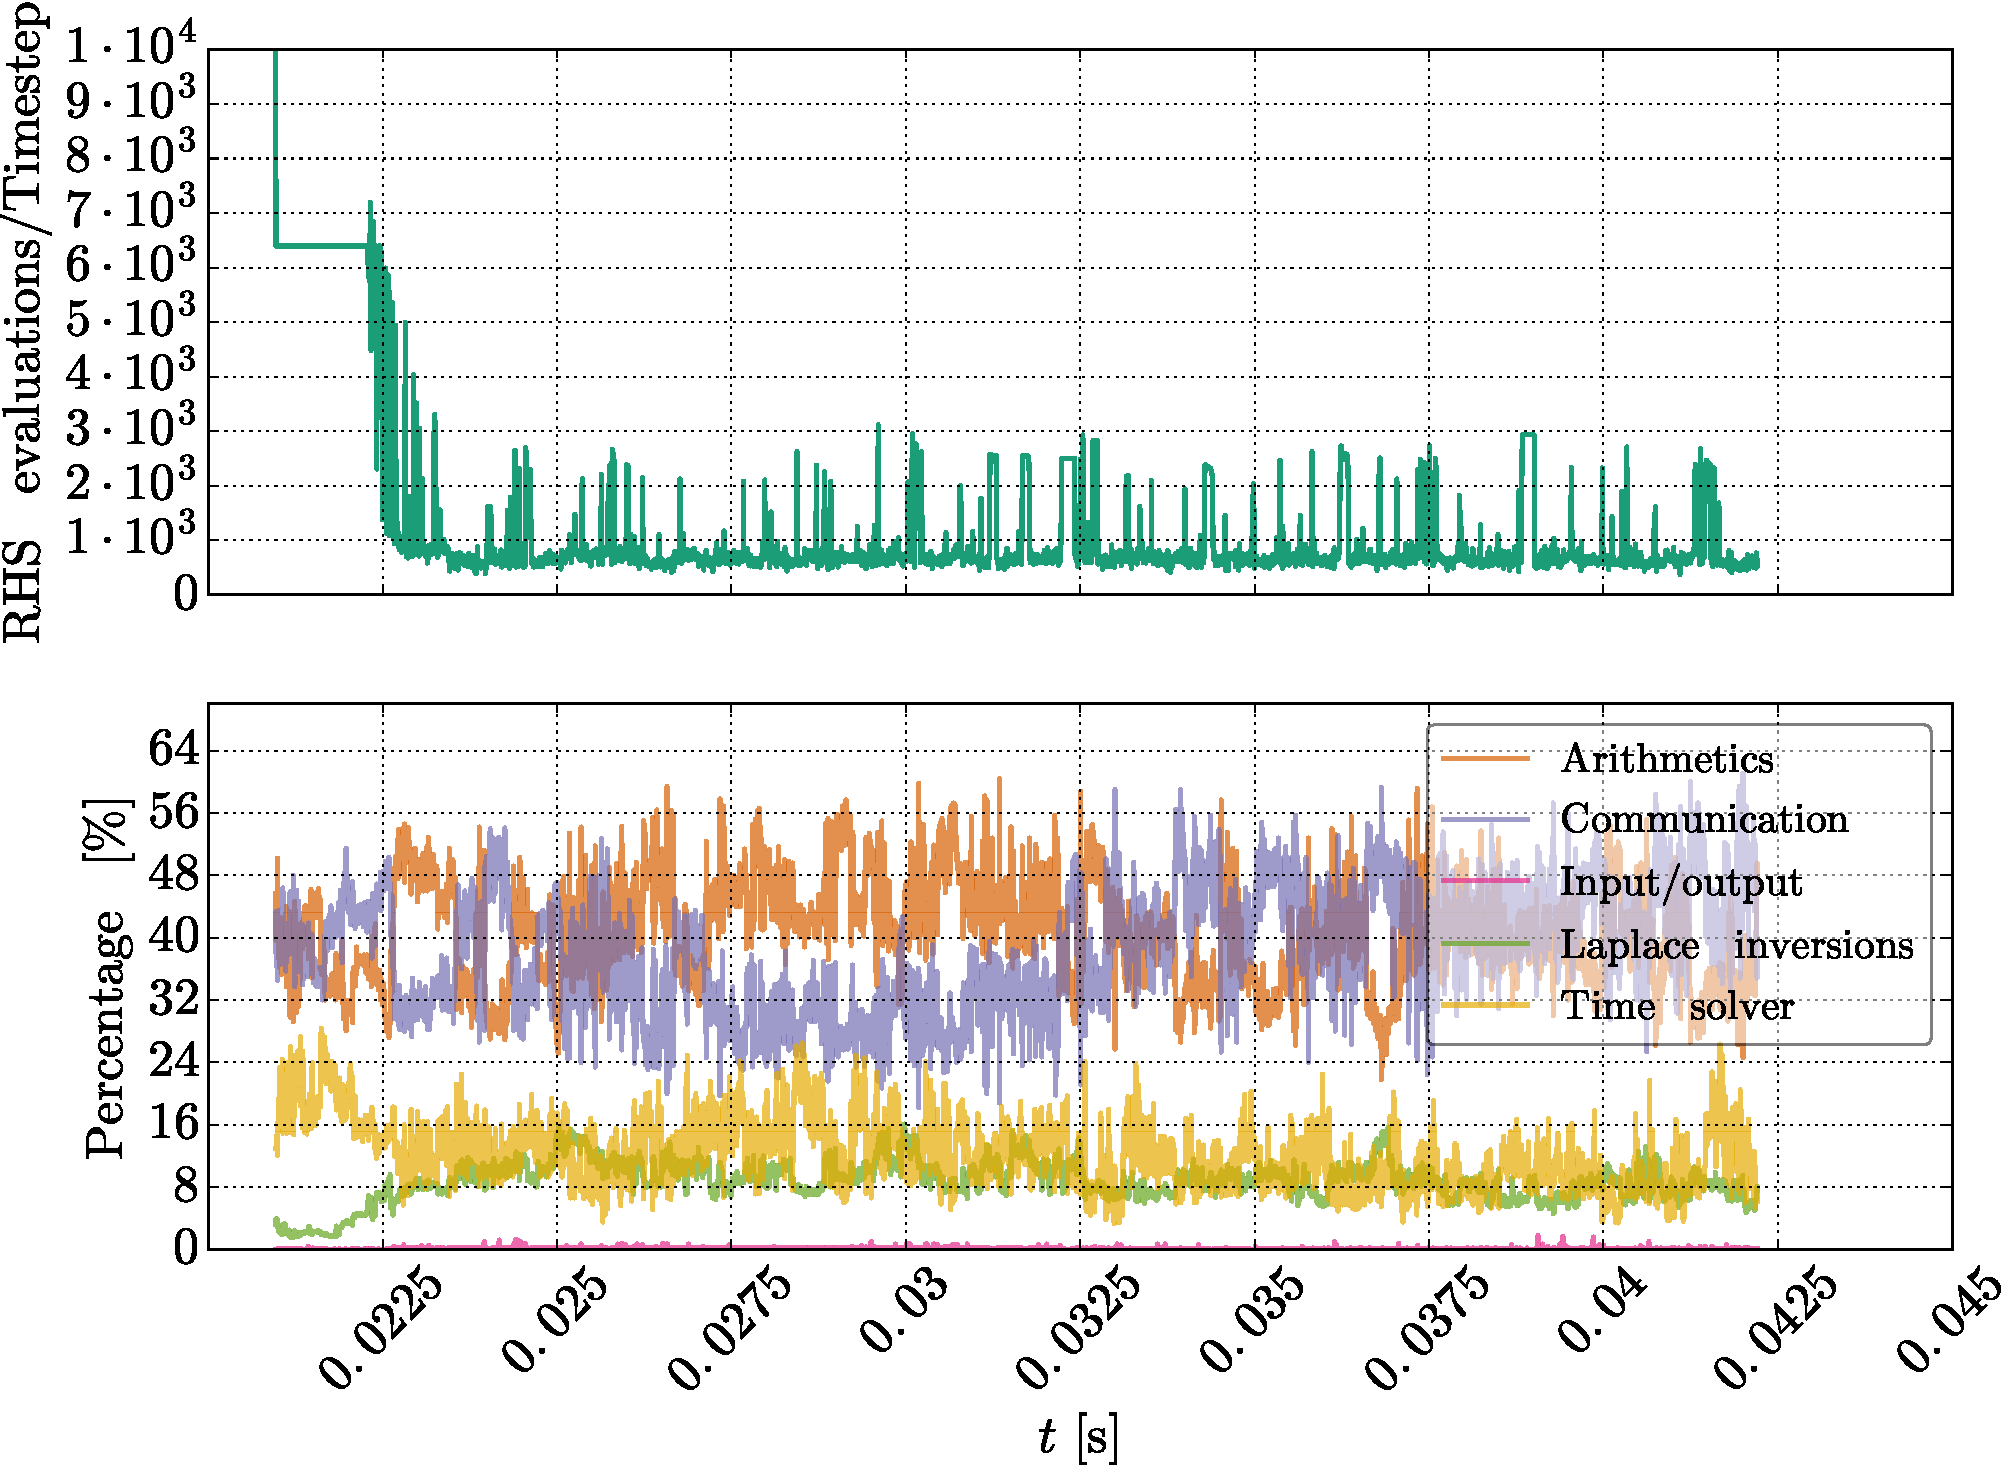
\includegraphics[width=1.0\textwidth]{fig/results/performance/performance008}
        \caption{$B=0.08\T$}
        \label{fig:perf008}
    \end{subfigure}
    \caption{Performance of the code.
        \cref{fig:perf004B,fig:perf006B,fig:perf008B} uses the Boussinesq approximation, whereas \cref{fig:perf004,fig:perf006,fig:perf008} does not.}
    \label{fig:perfB}
\end{figure}
%
Before the added perturbation, the simulations using the Boussinesq approximation uses around $100$ iterations per time step, whilst the non-Boussinesq model uses between $4000 - 12000$ iterations per time step.

In the non-Boussinesq case, the iteration count is almost constant, and higher than in the saturated turbulence case.

Most of the simulation time is done when communicating between processors and doing arithmetic operations on the fields for both models.
The time used in the external time solver (\texttt{cvode}) is always less than this.
In the Boussinesq case there is a significant increase of time used in both the communication process and the Laplace inversion (where the potential is solved from the vorticity).
This can be explained by the extra communication and inversion needed in the iterative Naulin solver, which uses between $3-10$ iteration per time step in the saturated turbulent phase.
